\section{Einleitung}\label{S:Intro}

Moderne Fahrsicherheits-, Fahrkomfort- oder Parkiersysteme wie Kollisionsvermeidung, Ausweich-, Nothalteassistenz, Spurhalteunterstützung, Stauassistenz und ferngesteuertes Einparken werden eingesetzt, um den Fahrer von seiner Fahraufgabe zu entlasten und das Fahren sicherer und komfortabler zu gestalten. 

In der industriellen Entwicklung der Fahrerassistenz in den beiden letzten Dekaden wurden in der Regel Einzelfunktionen mit begrenztem funktionalem Umfang und Betriebsbereich sowie individuellen Sicherheitskonzepten, Funktions-, Bordnetz- und Softwarearchitektur in Kooperationsmodellen mit unterschiedlichem Funktionsschnitt zwischen Fahrzeugherstellern und Lieferanten entwickelt.  
Zu Beginn legitim und vorteilhaft wegen der sehr unterschiedlichen Betriebsbereiche und sich abgrenzender Fahrfunktionen bzgl. Verantwortungsmodellen, Entwicklung, Applikation, Test und Absicherung mit großem funktionsindividuellem Handlungsspielraum wird dieses Vorgehen mit zunehmendem Überlappungsbereich der verschiedenen Assistenzfunktionen zum Problem der Komplexitätsbeherrschung.
Typischerweise wurden für Einzelfunktionen separate Reglerstrukturen entwickelt mit individuellen Funktionsschnitten auch zwischen Steuergeräten sowie zwischen OEM und Systemlieferanten. Um die zunehmende Vernetzung und Überlappung der Funktionen hinsichtlich Funktionsumfang und Betriebsbereich zu beherrschen ist es vorteilhaft, eine intergrierte  hierarchische Reglerstruktur zu entwickeln mit funktionsübergreifenden klaren Schnittstellen zu Sensorik und Aktuatorik und klaren Schnittstellen zwischen OEM und Systemlieferant.  


\subsection{Ziel des Beitrags}
Ziel des Beitrags ist es, einen Weg aufzuzeigen, durch einen strukturierten, hierarchischen modellbasierten regelungstechnischen Ansatz verschiedene Einzelsysteme der Fahrerassistenz zu einem integrierten Gesamtsystem zusammenzufügen.

\subsubsection*{Allgemeine Aufgabe}
Den Einzelfunktionen gemein ist, dass jeweils 
\begin{itemize}
\item ein Aktivieren der Funktion
\item ein Passivieren der Funktion bzw. der Übergang, die Transition, auf eine andere Funktion
\item das Führen des Fahrzeugs entsprechend einer definierten Fahraufgabe z.B. dem Führen entlang einer vorgegebenen Trajektorie mit den einzelnen Schritten
\begin{itemize}
\item Trajektorienplanung
\item Trajektorienfolgeregelung
\item Fahrzeugführungsregelung zur Überführung des Ergebnisses der Trajektorienfolgeregelung in Aktuatorstellgrößen
\end{itemize}
\end{itemize}
durchgeführt wird. Diese Schritte sind unabhängig davon, ob es sich hierbei um eine Längs-, Quer- oder kombinierte Quer-und Längsführungsaufgabe handelt.

\subsubsection*{Kooperationsgrade}
Fahrerassistenzsysteme unterscheiden sich in Ihrer Interaktion mit dem Fahrer. In der BAST~\cite{Gasser2012} wird unterschieden zwischen Level 1 - 5 ... assistiertes bis vollautomatisiertes Fahren. Hintergrund ist hier die Verantwortung, Haftung, Funktions-/Gebrauchssicherheit, Integrität der ....Aus einem regelungstechnischen Gesichtspunkt heraus ist diese Unterscheidung von untergeordneter Bedeutung.
Eine Level 1/2 Funktion bei der aus Sicht der funktionalen Sicherheit oder der Gebrauchssicherheit der Fahrer stets in der Überwachung bleibt, muss trotzdem der Regelkreis auch kurzfristige autonome Fahrzustände (bei Querführung z.B. \textit{handsoff} beherrschen, ohne instabil zu werden, ohne allzuviel Querablage aufzubauen, .... Wir lösen uns deswegen von der BAST-Definition und definieren nachfolgend drei Kooperationsgrade in der Mensch-Maschine-Schnittstelle:
\begin{itemize}
\item {\it Manuelles Fahren}: Das Fahrerassistenzsystem, der "Fahrroboter", ist abgeschaltet, der Fahrer führt das Fahrzeug bzgl. einer bestimmten Fahraufgabe (Längs- und/oder Querführung wie bspw. links oben in Abb.~\ref{fig:koopgrad} dargestellt.
\item {\it Autonomes Fahren}: Das Fahrerassistenzsystem, der Fahrroboter, führt das Fahrzeug bzgl. einer bestimmten Fahraufgabe (Längs- und/oder Querführung). Der Fahrer verhält sich passiv und ist mechanisch entkoppelt (\textit{handsoff}, \textit{feetoff}) wie bspw. rechts oben in Abb.~\ref{fig:koopgrad} dargestellt.
\item {\it Kooperatives Fahren}: Fahrerassistent und Fahrer führen kooperativ das Fahrzeug. Der Fahrer als auch der Fahrroboter sollen bei der kooperativen Fahrzeugführung die Führungsrolle übernehmen können. Der jeweils andere Partner schätzt/beobachtet dabei die Intention des Führenden ab und adaptiert sich daran. Zwei Fälle können wir hier unterscheiden. 
\begin{itemize}
\item Erstens, der Fahrer lässt sich gezielt führen und kann sehr stark reduziert als passive haptische mechanische Impedanz interpretiert werden die passiv mit dem Lenkrad oder dem (ggf. kraftreflektierenden) Fahr- oder Bremspedal verbunden ist wie bspw. links unten in Abb.~\ref{fig:koopgrad} dargestellt..  
\item Oder, zweitens, der Fahrer übernimmt die Führungsrolle mit einem in diesem Fall entsprechend nachgiebigem Fahrroboter- bzw. Fahrerassistenzsystem wie bspw. rechts unten in Abb.~\ref{fig:koopgrad} dargestellt. 
\end{itemize}
In der Robotik wird dieses Zusammenwirken von Mensch und Roboter mit {\it Human Robot Collaboration HRC} bezeichnet \cite{hrc_cite} und schließt die verschiedenen Ebenen der Wahrnehmung mit ein.  Wie gut das letztlich funktioniert hängt von den überlagerten High-Level-Navigations- oder Fahrstrategiefunktionen, der Qualität der Perzeption der Umgebung, der Gestaltung der Fahraufgabe, usw. ab. 
\end{itemize}
\begin{figure}[htp!]
  \centering
    \includegraphics[width=12cm]{Bilder/01/kooperationsgrade.eps}
    \caption{Kooperationsgrade dargestellt anhand der Querführung}
    \label{fig:koopgrad}
\end{figure}
Der Begriff des manuellen, kooperativen oder autonomen Fahrens kann selektiv für eine einzelne Funktion der Längs- oder Querführung verstanden werden. 
Manuelles Fahren längs kann bspw. kombiniert werden mit kooperativem Fahren quer (Spurhalteassistent), autonomes Fahren längs mit manuellem Fahren quer (ACC), usw. in allen sinnvollen Kombinationsmöglichkeiten.

Eine wichtige Rolle in der Gestaltung von kooperativen und autonomen Fahrfunktionen spielt auch die Einbindung des Fahrers in die Fahraufgabe über entsprechende Anzeige- und Bedienkonzepte. Eine Aktivierung und Passivierung einer Funktion muss gleichsam wie die Transition zu einer anderen Funktion oder auch die Aktion selber für den Fahrer über das Anzeige- und Bedienkonzept intuitiv begreifbar gemacht werden.
Hier gibt es keine prinzipielle Unterscheidung zu Einzelfunktionen.



%\begin{itemize}
%\item Kooperationsgrade einführen (manuell, kooperativ, autonom): 	Wie wird Fahrer eingebunden (Abschalt- / Transitionsstrategien mit Beispielen, Bedienung, ABK, Take-Over-Request, Abgrenzung zum Wettbewerb und zu Einzelfunktionen)
%\end{itemize}


%
%Ein geschlossener funktionaler Ansatz soll ... 
%
%\begin{itemize}
%	\item Mathematische Beschreibung des Betriebsbereichs
%	\begin{itemize}
%		\item Fahrgeschwindigkeit
%		\item Reibwert
%		\item Beladung
%	\end{itemize} 
%	\item Mathematische Beschreibung der Zustandsgrenzen
%	\begin{itemize}
%		\item Längs: Leistungshyperbel, Reibwert
%		\item Quer: Lenkwinkelendanschlag, Umfeldsensorik 
%					($\kappa_{max}$), Reibwert
%		\item Längs \ Quer: Kammscher Kreis
%		\item Kundensicht: reale Reibwertausnutzung
%	\end{itemize} 
%	\item Mathematische Beschreibung der Regelungsaufgabe
%	\begin{itemize}
%		\item Regelgüte: Führungs- und Störunterdrückungsverhalten, Dämpfung, Bandbreite, Stabilitätsreserve, 
%		\item Stabilität
%		\item Robustheit: Robust gute Regelgüte, Stabilität bei strukturierten und unstrukturierten Unsicherheiten 
%	\end{itemize}
%	\item Kooperationsgrade	
%	\begin{itemize}
%		\item Kooperationsgrade einführen (manuell, kooperativ, autonom): Wie wird Fahrer eingebunden (Abschalt- / Transitionsstrategien mit Beispielen, Bedienung, ABK, Take-Over-Request, Abgrenzung zum Wettbewerb und zu Einzelfunktionen)
%	\end{itemize}
%	\item Kundenfunktionen Level 2
%	\begin{itemize}
%		\item Längs: ACC, iBrake, Park-Assistenz
%		\item Quer: LSA, LCA, AWA
%	\end{itemize}
%\end{itemize}
\subsubsection*{Beriebsbereich}
Der Betriebsbereich von Fahrerassistenzfunktionen wird durch verschiedene limitierende Faktoren bspw. in Form von Stellgrößenbeschränkungen und Fahrzustandsgrenzen begrenzt. 
Hintergrund sind Stellgrenzen der Aktuatoren (z.B. Momenten-, Leistungsgrenzen), der Stellgrößen (Lenkwinkelendanschlag), der Sensorik (Krümmungsbeschränkung durch eingeschränktes Sichtfeld bei Umfeldsensorik), der Umgebung Reifen/Fahrbahnkontakt (Kamm'scher Kreis) aber auch Beherrschbarkeitsgrenzen die durch Aspekte der Funktions- und Gebrauchssicherheit vorgegeben werden oder vorgegebene Grenzen der funktionalen Ausprägung (z.~B. Ruckbegrenzung bei Komfortfunktionen). In den regelungstechnischen Entwurf können diese durch geeignete Zustands-, Eingangs-, Ausgangs- oder Parametergrenzen die den zulässigen Bewegungsraum einschränken berücksichtigt werden.
Beispielhaft zeigt hierzu Abb.~\ref{fig:bew_lims} die Bewegungsgrenzen für die Längsführung (links) und der Querführung (rechts) für unterschiedliche Assistenzfunktionen und allgemein für das manuelle Fahren. Abgebildet im Diagramm ist für die Längsführung eine Ruckbegrenzung für den stillstandsnahen Bereich, eine Beschleunigungsbegrenzung aufgrund des Kamm'schen Kreises oder auch aufgrund Beherrschbarkeit oder funktionaler Ausprägung und eine Antriebsleistungsbegrenzung in Form einer Hyperbel. Für die Querführung wurde zusätzlich der Lenkwinkelendanschlag im stillstandsnahen Bereich in Form einer Parabel dargestellt.
  
%%\begin{itemize}
%%\item Sensorgrenzen: Krümmungsbegrenzung aufgrund	...
%%\item Stellgrößenbeschränkungen
%%	- Aktuatorgrenzen
%%		- Stellbeschränkungen
%%		- Stellratenbeschränkungen
%%	- Lenkwinkelendanschlag
%%\item Fahrzustandsgrenzen
%%	- Grenzen der Fahrphysik
%%		- Kamm'scher Kreis
%%	- Komfortgrenzen
%%		- Ruckbegrenzung
%%		- Beschleunigungsbegrenzung quer/längs
%%	- Sicherheitsgrenzen			
%%		- Ruckbegrenzung
%%		- Beschleunigungsbegrenzung quer/längs
%%\item Grenzen der Beherrschbarkeit aus Sicht der funktionalen Sicherheit und der Gebrauchssicherheit
%%	- Momentengrenzen Quer-/Längs
%%\end{itemize}
\begin{figure}[htp!]
  \centering
    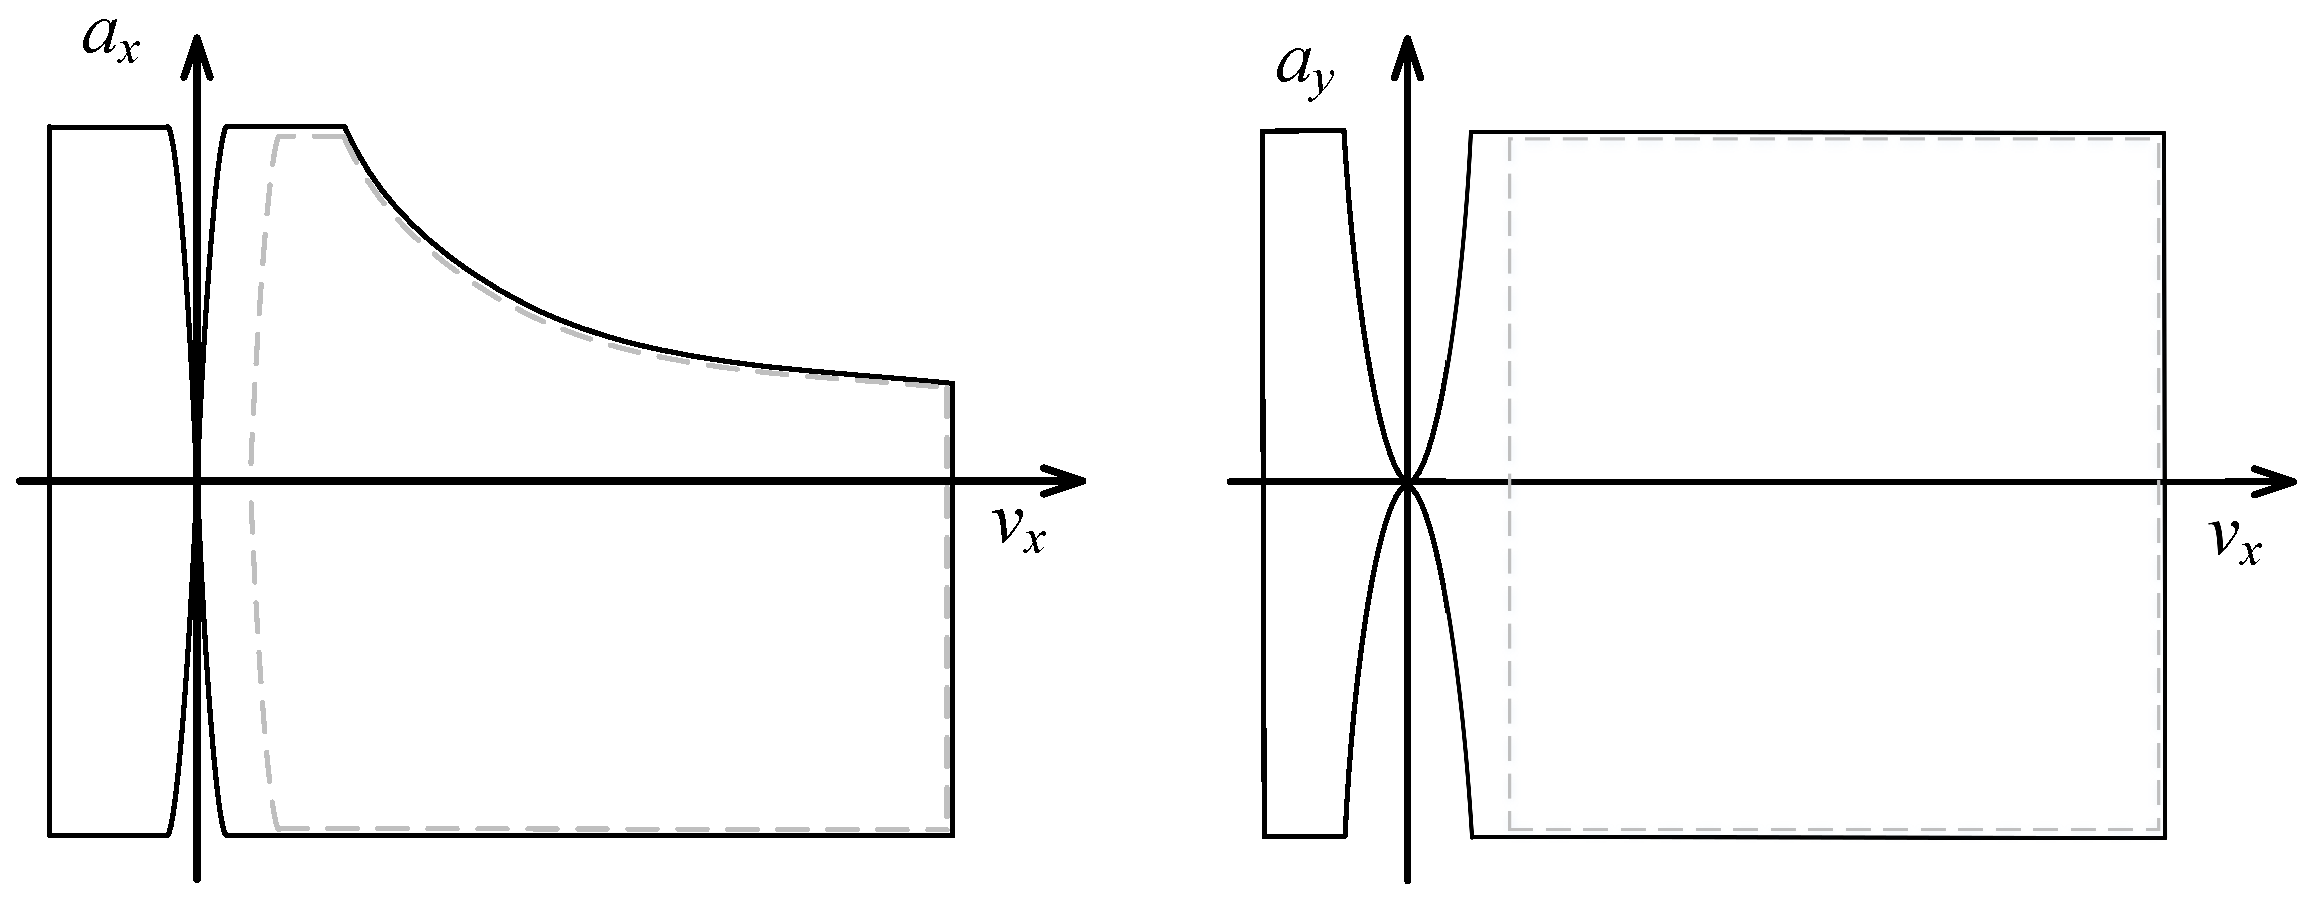
\includegraphics[width=10cm]{Bilder/01/betriebsbereich.eps}
    \caption{Quasistationäre Bewegungsgrenzen für Längs- und Querführung (manuelles Fahren, Ausweichassistent, ACC, Parkierassistent, Nothalteassistent)}
    \label{fig:bew_lims}
\end{figure}

Weiterhin müssen die Fahrerassistenzfunktionen bei variierenden Betriebsparametern bspw. einer von Fahrt zu Fahrt variierenden unbekannten Zusatzbeladung des Fahrzeugs, einer aufgrund eines Reifenwechsels unbekannten Bereifung, dem witterungsbedingt unsicheren Reifen-/Fahrbahnzustand, in einem unterschiedlich großen Fahrgeschwindigkeitsbereich gleichermaßen gut d.~h. robust gut funktionieren. Natürlich ist es möglich, verschiedene Einflußgrößen hierbei während der Fahrt zu schätzen bzw. zu beobachten und die Assistenzfunktion daran zu adaptieren.  
Abb.~\ref{fig:m_vert} zeigt hierzu exemplarisch den Einfluss einer zu berücksichtigenden Zusatzbeladung und deren Positionierung. Diese ergibt sich beispielsweise aus unterschiedlichen Derivaten, Motorisierungen, Sonderausstattungen innerhalb einer Produktlinie, der Zusatzbeladung selbst durch eine unterschiedliche Anzahl von Personen im Fahrzeug, Dachträger, Kofferraum, etc.. Ein Fehlermodell der Zusatzmasse wird erstellt welches ihren Einfluss auf die Fahrzeugparameter bspw. die Schwerpunktlage, Masse oder Träghheitsmomente beschreibt.  
%\begin{itemize}
%	\item Mathematische Beschreibung des Betriebsbereichs
%	\begin{itemize}
%		\item Fahrgeschwindigkeit
%		\item Reibwert
%		\item Beladung
%	\end{itemize} 
%\end{itemize} 
\begin{figure}[htp!]
\centering
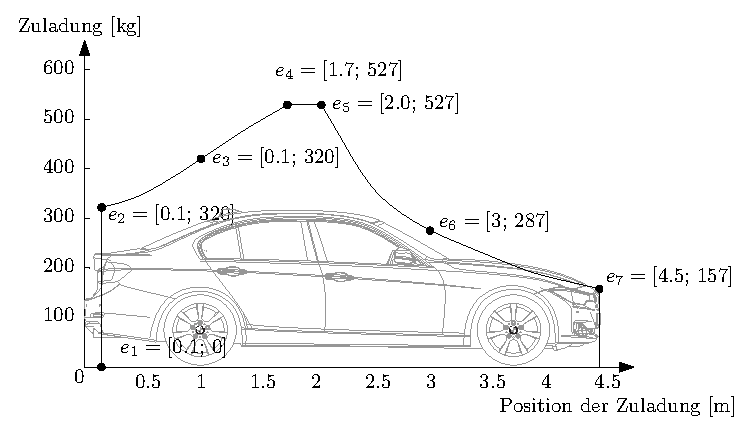
\includegraphics[width=8cm]{Bilder/01/massen_verteilung_f30.eps}
\label{fig:m_vert}
\end{figure}


%\subsubsection*{Grenzen}

%\begin{figure}[htp!]
%%  \centering
%    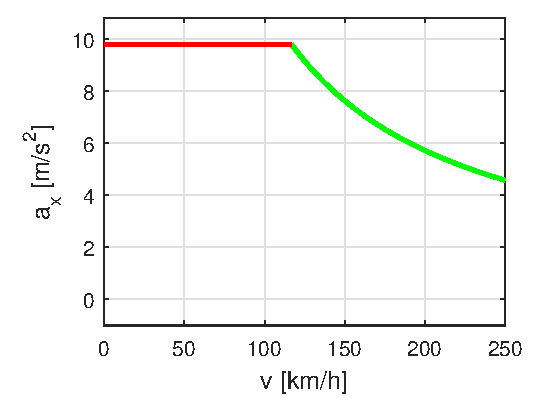
\includegraphics[scale=0.6]{Bilder/01/v_ax.eps}
%    \hspace{1cm}
%%   \caption{Grenzen L.}
%%   \label{fig:v_ax}
%%\end{figure}
%%\begin{figure}[htp!]
%%  \centering
%    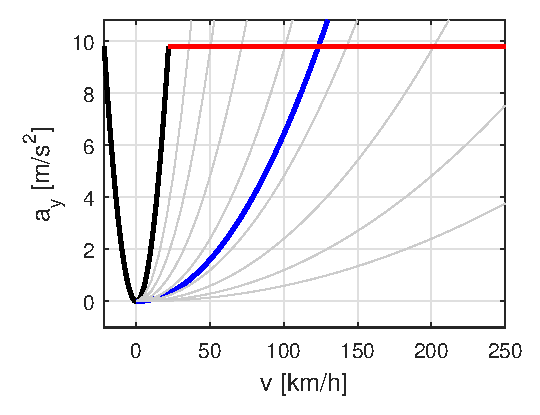
\includegraphics[scale=0.6]{Bilder/01/v_ay.eps}
%    \caption{Grenzen Längsdynamik}
%    \label{fig:v_ay}
%\end{figure}

\subsubsection*{Regelungsaufgabe}
Die modellbasierte Regelung MBC (\textit{Model Based Control}) 
entstand in den 1960er Jahren durch die Einführung des Zustandsraummodells durch Kalmann zusammen mit \textit{Optimal Control} 
und beinhaltet heute eine Vielzahl von Methoden für die Regelung von linearen und nichtlinearen Systemen. In einer Vielzahl von Anwendungen bspw. in der Flugregelung, der    
Robotik, der Vertikaldynamikregelung, der Fahrdynamikregelung, der Antriebsregelung, der Aktuatorregelung oder der Regelung im Zusammenhang mit Fahrerassistenzsystemen der Längs- und Querführung werden MBC Methoden heute sehr erfolgreich eingesetzt. Lineare Methoden beinhalten beispielsweise LMI, IMC, Polvorgabe, LQR, quasilineare Methoden wie die Popov-Methode oder das Zweiortskurvenverfahren sowie nichtlineare Methoden bspw. Lypunov-basierte Methoden oder Ein-/Ausgangslinearisierung.  Gemeinsame Grundlage für den erfolgreichen industriellen Einsatz dieser Methoden ist, dass ein einfaches physikalisches Modell der Regelstrecke existiert und Abweichungen von diesem Modell durch entsprechende mathematische Unsicherheitsmodelle beschrieben werden können. 
%Zunächst für den Entwurf in Form von parametrischen linearen/nichtlinearen zeitinvarianten Systemen in Zustands- oder Übertragungsform (\textit{linear parametric LTI system}), 
%numerisch linearer parametervariierender Systeme (\textit{LPV systems}), 
%additive oder multiplikative Unsicherheitsmodelle im Frequenzbereich (\textit{additive or multiplicative perturbation models}).
Für die Anwendung der integrierten Quer- und Längsführung haben sich aufgrund der Aufgabenstellung insbesondere lineare Verfahren mit einer ....  bewährt.
 
Die Regelungsaufgabe soll beschreiben welche Eigenschaften der geschlossene Regelkreis besitzen soll. Dies umfasst, dass der Regelkreis zunächst grundsätzlich stabil sein soll,
 d.~.h dass die Reaktion des geschlossenen Regelkreises auf externe Anregungen nicht zu einem instabilen Verhalten führt. Insbesondere sind hierbei Aspekte die durch numerische Diskretisierungsverfahren, Multirating, Quantisierungen, Totzeiten, Lose, Reibungseffekte, Sensorrauschen oder Strukturvariabilität im Stellprinzip(VDDS) zu beachten und bei Bedarf in der regelungstechnischen Synthese zu berücksichtigen.

Wesentliche Aufgabe ist es, ein gutes Führungs- und Störübertragungsverhalten zu realisieren. In unserem Fall bedeutet dies, dass Sollvorgaben für den Regelkreis durch eine Trajektorienplanung skalierbar steif und stationär genau eingeregelt werden können sollen. Störungen beispielsweise induziert durch Seitenwind, Reibwertsprünge sollen kompensiert werden.

Die Eigenschaften der Stabilität und des guten Führungs- und Störübertragungsverhaltens sollen robust sein gegenüber variierenden nicht mess-/schätz-/beobachtbaren Parametern und Fahrzustandsgrößen, gegenüber im Regelungsentwurf nicht berücksichtigten Modellierungsungenauigkeiten und beispielsweise nichtlinearen Effekten wie oben beschrieben.   


%Dies schließt auch die Vermeidung von nichtlinearer Grenzzyklen (Grenzschwingungen), häufig induziert durch nichtlineare  
  
%\begin{itemize}
%\item \emph{Stabilität} Zunächst muss Stabilität für das Gesamtsystem sichergestellt werden. Zum einen   
%Stabilität, asymptotische Stabilität nach Lyapunov
%absolute Stabilität Vermeidung nichtlinearer Grenzzyklen (Grenzschwingungen) in der Gegenwart von Nichtlinearitäten
%Vermeidung driver induced oscillations. Eine Überreaktion des Fahrers oder eine zeitlich ungünstig versetzte Reaktion des Fahrers kann zu ungewünschten Schwingungsphänomenen führen 
%
%\item \emph{Regelgüte} Führungs- und Störübertragungsverhalten im Sinne von schneller Einschwingzeit des Regelkreises
%
%\item \emph{Robustheit}
%\end{itemize}  
% 
% Diskretisierung, multirating, Totzeiten, Lose, Reibungsmodell, Sensorrauschen., strukturvariable Systeme (VDD)... 
%
% 
% Regelgüte
% 
% Robustheit der Eigenschaften Stabilität und Regelgüte bei variierenden Betriebsparametern
% Robustheit gegenüber nichtmodellierten Dynamiken
% 
Zusätzlich zum Fahrversuch bietet es sich an analytische Struktureignungsanalysen und simulativ gestützte Analysen mit komplexeren Fahrzeug-, Sensorik-, Aktuatorik- und Umgebungsmodellen durchzuführen.
 
 
 

%\subsubsection*{Kundenfunktionen}
%
%
%
%
%\begin{figure}[htp!]
%\centering
%\includegraphics[width=12cm]{Bilder/01/KoordSys.pdf}
%\end{figure}
%
%
%
%%\begin{figure}[htp!]
%%\centering
%%\import{Bilder/01/}{Impedanzmodell_Lenkung.pdf_tex}
%%\caption{Grundstruktur des Störgrößenbeobachters mit Kompensation}
%%\label{fig:01_Lenkung}
%%\end{figure}
%
%%\begin{figure}[htp!]
%%\centering
%%\import{Bilder/01/}{Impedanzmodell_Lenkung_visio.pdf_tex}
%%\caption{Grundstruktur des Störgrößenbeobachters mit Kompensation}
%%\label{fig:01_Lenkung}
%%\end{figure}
%
%
%Ruckbegrenzung bei unterschiedlichen Anfangsgeschwindigkeiten
%
%
%
%
%\begin{figure}[htp!]
%  \centering
%    \includegraphics[scale=0.83]
%    {Bilder/01/Impedanzmodell_Lenkung.eps}
%    \caption{Kooperative Fahrzeugführung mit Regelstrecke für Querführung mittels Lenkung.}
%    \label{fig:Imp_Lenkung}
%\end{figure}
%
%\begin{figure}[htp!]
%  \centering
%    \includegraphics[scale=0.83]
%    {Bilder/01/Impedanzmodell_Quer.eps}
%    \caption{Kooperative Fahrzeugführung mit Regelstrecke für Querführung.}
%    \label{fig:Imp_Lenkung}
%\end{figure}
%
%\begin{figure}[htp!]
%  \centering
%    \includegraphics[scale=0.83]
%    {Bilder/01/Impedanzmodell_FF.eps}
%    \caption{Kooperative Fahrzeugführung mit Regelstrecke für Quer- und Längsführung.}
%    \label{fig:Imp_Lenkung}
%\end{figure}
%
